\chapter{畳み込みニューラルネットワーク(CNN:Convolutional Neural Network)}
\section{CNNの概要}
この章では、FiC-SW1の予備評価のためにベンチマークアプリケーションとして実装する畳み込みニューラルネットワーク(CNN:Convolutional Neural Network、以下CNN)について解説する。

CNNは、主に画像識別に用いられる順伝搬型ネットワークの一種である。
順伝搬型ネットワークは前の層と後ろの層が互いに全対全で結びつく全結合が一般的だが、
CNNではカーネルと呼ばれるフィルタを導入して結合に局所性を持たせている。
これにより、全結合に比べ計算処理を減らし、効率的に処理を行うことが可能となった。

図\ref{fig_cnn}に一般的な画像識別を行うCNNの推論の概要を示す。
CNNでは2次元画像データのことを特徴マップと呼び、特徴マップに対してカーネルを用いて畳み込み演算を行う畳み込み層と、
一定の範囲から値を絞るプーリング層の2種の層を組み合わせるのが構成と成っている。
畳み込み層は、カーネルと同じパターンが画像のどこに存在するかを判定する効果がある。
プーリング層は画像に写っている対象の位置感度を低下させ、位置に対する依存性を低くする効果がある。

また、ほとんどの場合において、畳み込み層は識別層の前に設けられる。
これは、複数の畳み込み層、プーリング層を組み合わせることで、識別層の入力値の数を絞り込み、
識別層の処理の負荷を軽くする狙いがあるからである。

さて、学習の処理では、教師データを用いて誤差逆伝搬法によって、畳み込み層と識別層の重みを繰り返し再計算していく形となる。
今回扱うのはこのようなCNNの推論処理のみなので、学習処理については詳しくは扱わないこととする。

\begin{figure}[ht]  
 \begin{center}   
	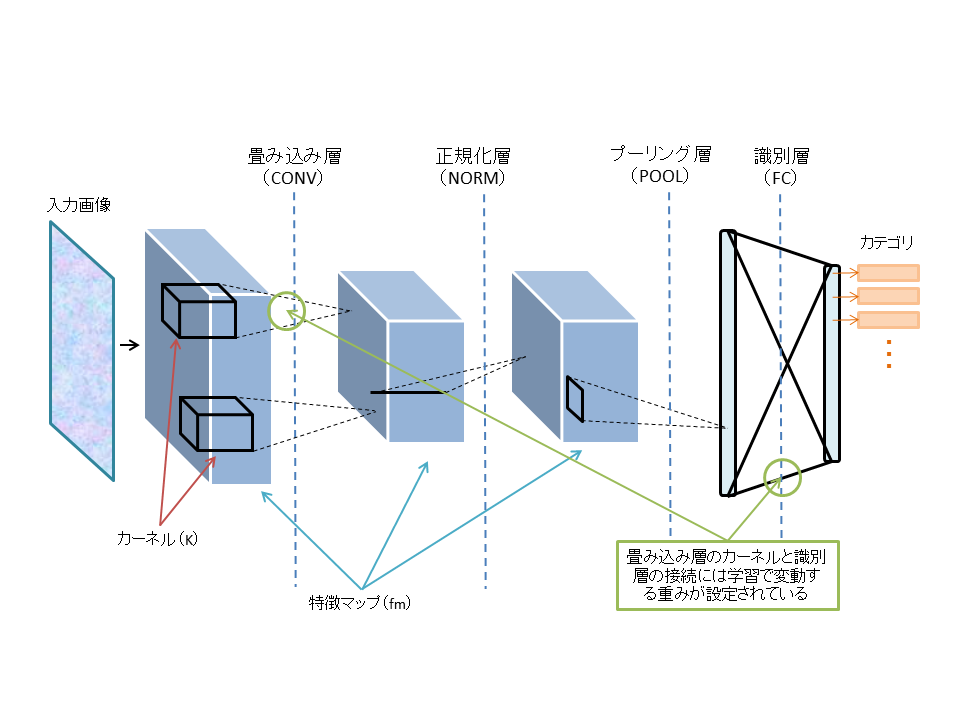
\includegraphics[width=1.0\columnwidth,bb=0 0 720 540]{img/cnn.png}
    \caption{畳み込みニューラルネットワークの推論}
%  \ecaption{Static analysis result of an example pattern}
  \label{fig_cnn}  
 \end{center}  
\end{figure}


\section{畳み込み層の処理}
CNNの特徴のひとつである畳み込み層は、入力特徴マップに対してフィルタの役割を持つカーネルを用いて畳み込み演算を行い、特徴を抽出するためのレイヤーである。

\subsection{畳み込み演算}
図\ref{fig_conv}は、畳み込み層の最も重要な処理である畳み込み演算について解説したものになる。畳み込み演算の処理は画像のフィルタリングに似ており、
N次元の入力特徴マップとN次元のカーネルの行列演算の結果を出力特徴マップの値として出力する。
カーネルの範囲K×Kは、横方向にずらしていき、端まで到達したら縦方向に
ずらしてから同様に横方向に移動させていく。このように左上から右下へとフィルタリングした結果が1枚の出力特徴マップとなる。
さらに、カーネルはM枚(チャンネル)存在し、出力特徴マップもカーネルによってM枚(チャンネル)に分かれることになる。
つまり、入力特徴マップN枚とカーネルM×N枚から出力特徴マップM枚を計算するのが畳み込み演算である。

また、畳み込み層のカーネルにはそれぞれ重みが与えられており、これが学習で変動する。つまり、M×N×K×Kが重みデータの総量となる。
さらに、畳み込み層には学習で変動するバイアス(bias)のデータが存在する。これは畳み込み演算終了後に対応する出力特徴マップに加算する数値で、
出力特徴マップのチャンネル別にM個のデータがある。


\begin{figure}[ht]  
 \begin{center}   
	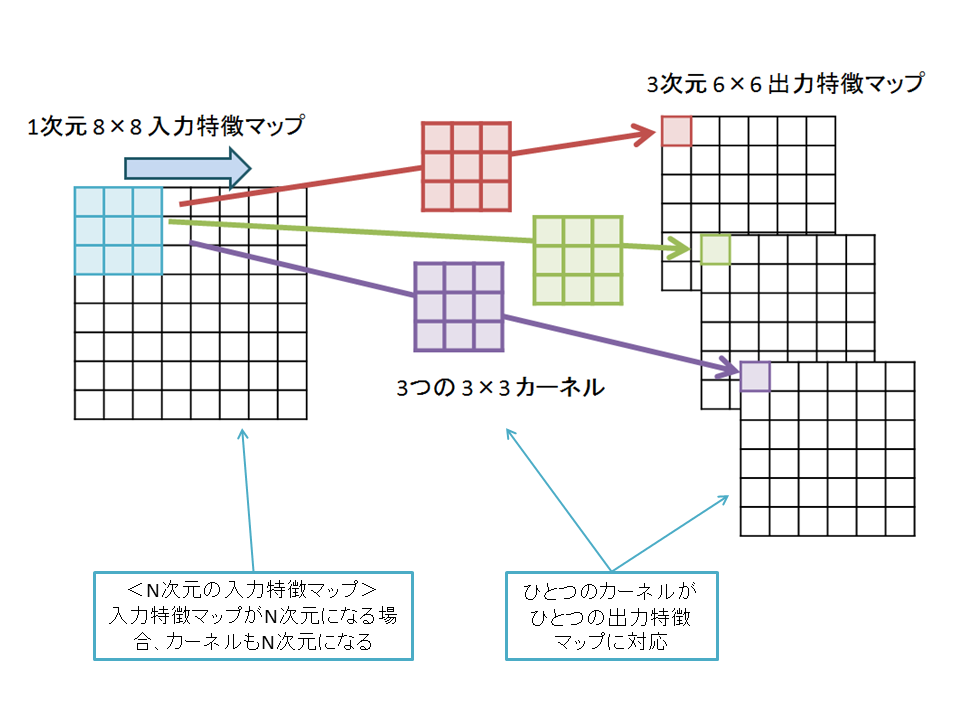
\includegraphics[width=1.0\columnwidth,bb=0 0 720 540]{img/conv.png}
    \caption{畳み込み層の演算}
%  \ecaption{Static analysis result of an example pattern}
  \label{fig_conv}  
 \end{center}  
\end{figure}

畳み込み演算を数式で表すと以下のようになる。

\[
  output(tr, tc)^{to} = \sum_{ti=0}^{N} \sum_{i=0}^{K} \sum_{j=0}^{K} weight_{to, ti}(i, j) * in(S * tr + i, S * tc + j)^{ti}
\]

このように、フィルタリング処理と同様、畳み込み演算は大規模な積和演算として捉えることができる。また、この演算を擬似コードで表すと以下のようになる。
コードを見るとわかるように、このデータ処理では、出力特徴マップのデータ間ではデータ並列性が存在するため、
並列演算器によって高速化できる余地があることがわかる。
このことは今回の畳み込みアクセラレータの実装を検討する上で最も重要な事実となる。

\begin{itembox}[1]{畳み込み演算のCコード}
\begin{verbatim}
for (int tr = 0; tr < R; tr++)
  for (int tc = 0; tc < C; tc++)
    for (int to = 0; to < M; to++)
      for (int ti = 0; ti < N; ti++)
        for (int i = 0; i < K; i++)
          for (int j = 0; j < K; j++)
            output[to][tr][tc] +=
              input[ti][S*tr+i][S*tc+j] *
              weight[to][ti][i][j];
\end{verbatim}
\end{itembox}

\subsection{活性化関数}
さて、畳み込み層ではもうひとつ重要な処理が行われる。それは畳み込み演算の結果を活性化関数と呼ばれる関数にかける処理である。
活性化関数は畳み込み演算の結果を正規化する目的で行われる計算で、正規化線形関数(ReLU : Rectified Liner function)やシグモイド関数などが使われる。

たとえば、最も一般的な正規化線形関数は数式にすると以下のようになる。

\[
  f(u) = max(u, 0)
\]

この関数は他の関数に比べ、処理が単純で、入力の変動が大きさに対して寛容なため、近年のニューラルネットワークで使われる機会が多い。

\section{その他の層の演算}
今回は畳み込み層の処理を主なベンチマークとして扱うが、CNNには他にもプーリング層や正規化層、識別層が存在している。ここではそれらの層の処理について解説する。

プーリング層(POOL)では、主に特徴の位置感度を低下させる目的で、最大値プーリング(maxpooling)や平均値プーリングが行われる。
たとえば、最大値プーリングでは、プーリングの範囲P×Pの中で最も大きい値を抽出し、出力とする。P×Pの範囲が大きいほど特徴マップのサイズは
小さくなって出力されることになる。

正規化層(NORM)では、画像のコントラストや露出の影響を抑え、識別の精度をあげる目的で設置される。
ここでは局所コントラスト正規化(LRN : Local Response Normalization)を解説する。

LRNはAlexNetの正規化層で用いられる処理で、数式で表すと以下のようになる。

\[
  output(x, y)^{i} = input(x, y)^{i} / (k + \alpha \sum_{j=max(0, i-n/2)}^{min(N-1, i+n/2)} (a^j_{x, y})^2)^\beta
\]

k、n、$\alpha$、$\beta$がパラメータであり、たとえば、AlexNetの正規化層では、k=1、n=5、$\alpha$=?、$\beta$=?となっている。

識別層(FC)は純粋な順伝搬型ニューラルネットワークであり、
すべての入力値と出力値の間に重みとバイアスが与えられている全結合の形になっている。
この重みは畳み込み層の重み・バイアスと同様、学習によって変動する。
畳み込み層、プーリング層、正規化層を経て抽出さえた値はこの識別層によって
最終的な分類が行われる。

識別層の処理を数式で表すと以下のようになる。

\[
  output(i) = bias(i) + \sum_{j=0}^{N} weight(i, j) * input(j)
\]

\section{大規模な画像識別CNN : AlexNet}
AlexNet\cite{alexnet}はImageNet2012で発表され、現在のCNNの基礎となっている一般的な
画像識別ニューラルネットワークのひとつである。
5つの畳み込み層、3つのプーリング層、2つの正規化層、3つの識別層(全結合層)から成る
このCNNは、227×227ピクセルのカラー画像を1000のカテゴリに分類することができる。
図\ref{imagenet_img}はAlexNetの全体の流れを示している。

今回はこのAlexNetの畳み込み層の推論(順伝搬)をベンチマークアプリケーションとして扱う。
表\ref{imagenet}は今回利用するAlexNetの各層のパラメータをまとめたものである。
Nは入力特徴マップの次元数、Mは出力特徴マップの次元数、R、Cは出力特徴マップサイズ、Kはカーネルサイズ、Sはストライド、padはパディングのパラメータとなる。
パディングとは畳み込み演算を行う前に、入力特徴マップの周りを0で埋める操作である。

一般的に畳み込み層はCONV、プーリング層はPOOL、正規化層はNORM、識別層はFCと略され、後ろに
その層が何層目にあたるかの数字をつけて区別する。

実際に2012年に発表されたAlexNetでは、CONV1、CONV2、CONV5は独立した2つのグループに分けられていた。
たとえば、CONV1の出力特徴マップは前半48層と後半48層といったように半分に分けられる。
しかし、今回の実装ではそれをひとつに結合したものを扱う。AlexNetがこのような2つのグループに
分かれていたのは、2つのGPUで処理を分担する都合上であり、それをひとつのシステム上で処理できるならば
ひとつのグループにまとめてしまっても問題はないためである。

\begin{figure}[ht]  
 \begin{center}   
	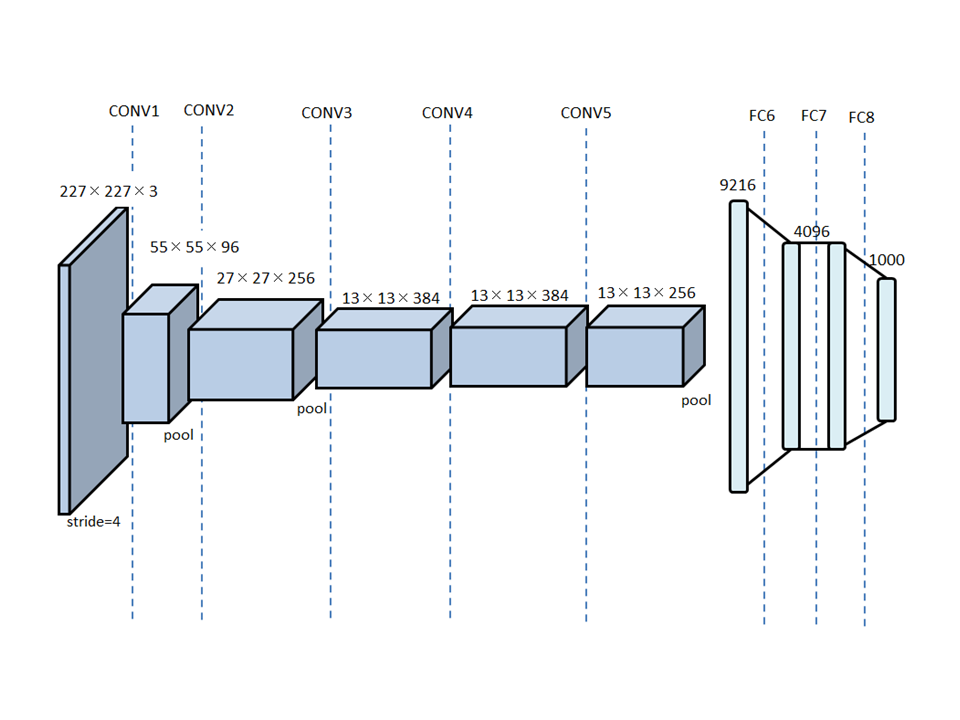
\includegraphics[width=1.0\columnwidth,bb=0 0 720 540]{img/imagenet.png}
    \caption{AlexNet\cite{alexnet}の概要}
%  \ecaption{Static analysis result of an example pattern}
  \label{imagenet_img}  
 \end{center}  
\end{figure}

\begin{table}[ht]
 \begin{center}
  \caption{AlexNetの各層の詳細なパラメータ}
   \begin{tabular}{|c|c|c|c|c|c|c|} \hline
     層 & 入力fm N & 出力fm M & サイズ(R,C) & カーネルK & ストライドS & パディング \\ \hline
     CONV1 & 3 & 96 & 55 & 11 & 4 & 0 \\
     NORM1 & 96 & 96 & 55 & - & - & - \\
     POOL1 & 96 & 96 & 27 & 3 & 2 & - \\
     CONV2 & 96 & 256 & 27 & 5 & 1 & 2 \\
     NORM2 & 256 & 256 & 27 & - & - & - \\
     POOL2 & 256 & 256 & 27 & 3 & 2 & - \\
     CONV3 & 256 & 384 & 13 & 3 & 1 & 1\\
     CONV4 & 384 & 384 & 13 & 3 & 1 & 1\\
     CONV5 & 384 & 256 & 13 & 3 & 1 & 1\\
     POOL5 & 256 & 256 & 6 & 3 & 2 & - \\
     FC6 & 9216 & 4096 & - & - & - & - \\
     FC7 & 4096 & 4096 & - & - & - & - \\
     FC8 & 4096 & 1000 & - & - & - & - \\ \hline
  \end{tabular}
  \label{imagenet}  
 \end{center}
\end{table}
